\section{Modelos em \LaTeX}

\begin{frame}
    Uma das facilidades do \LaTeX é  permitir que vários arquivos textos seja incluídos/importados no documento final, permitindo que um mesmo documento seja composto por vários arquivos texto.\\
    Para fazer uma inclusão de um arquivo externo, basta inserir uma das seguintes linhas:

\vspace{1cm}
\begin{center}
    {\ttfamily \textbackslash input {pasta/arquivo}}\\
    {\ttfamily \textbackslash input\{pasta/arquivo2\}}
\end{center}

\end{frame}


\begin{frame}
\subsection*{Modelos padronizados em \LaTeX} % (fold)

Na produção científica é comum a publicação de trabalhos em modelos já  prontos em \LaTeX~que já formatem automaticamente todo o texto de acordo com um padrão pré-determinado, esse modelos são amplamente utilizados em trabalhos como TCC, tese, dissertação, relatório e publicação de artigos em revistas. Alguns exemplos de podem ser encontrados no site:

\begin{center}
\url{https://www.sharelatex.com/templates/journals}
\end{center}
\end{frame}


\begin{frame}
Utilizaremos dois {\it templates}, o {\it journal Procedia Computer Science} da editora \textbf{Elsevier} para publicação de artigos, e o relatório de engenheiros para o exercito americano {\it Reports by US army of Corps Engineers} .

Execute o arquivo {\ttfamily conteudo.tex} e {\ttfamily info.tex} presente na pasta na raiz do diretório de templates.
\begin{figure}
\begin{center}
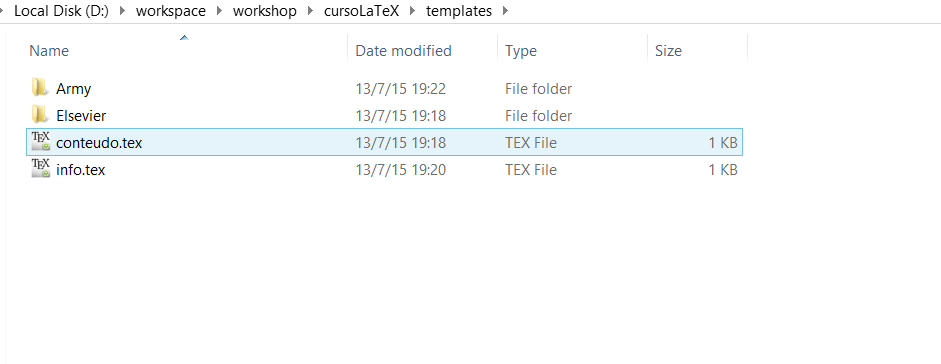
\includegraphics[scale=0.5]{figuras/template-dir.png}
\caption{Diretório de templates}
\end{center}
\end{figure}
\end{frame}

\begin{frame}
Fizemos imports de maneira a facilitar a elaboração de relatórios/papers/etc tendo o mesmo conteúdo mas tendo saídas em templates e padrões diferentes. Dessa maneira, basta editar o arquivo {\ttfamily conteudo.tex} com o corpo do texto, e o {\ttfamily info.tex} com as informações de autores e etc.
\begin{figure}
\begin{center}
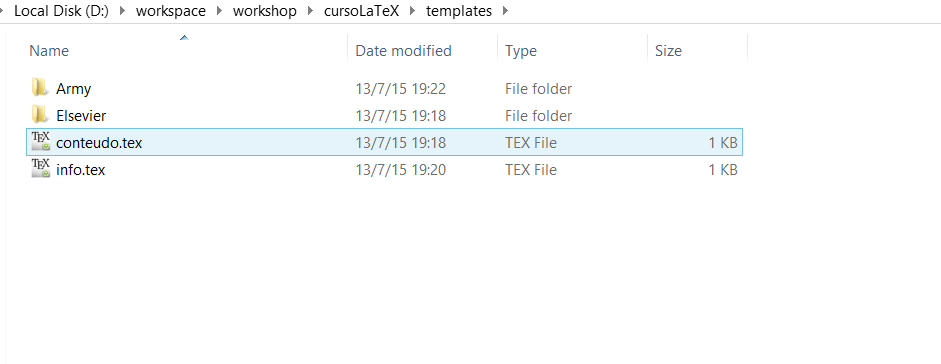
\includegraphics[scale=0.5]{figuras/template-dir.png}
\caption{Diretório de templates}
\end{center}
\end{figure}
\end{frame}

\begin{frame}

\begin{figure}
Observe os comandos de \textbackslash input e \textbackslash bibliography nos arquivos tex internos de cada template:
\begin{center}
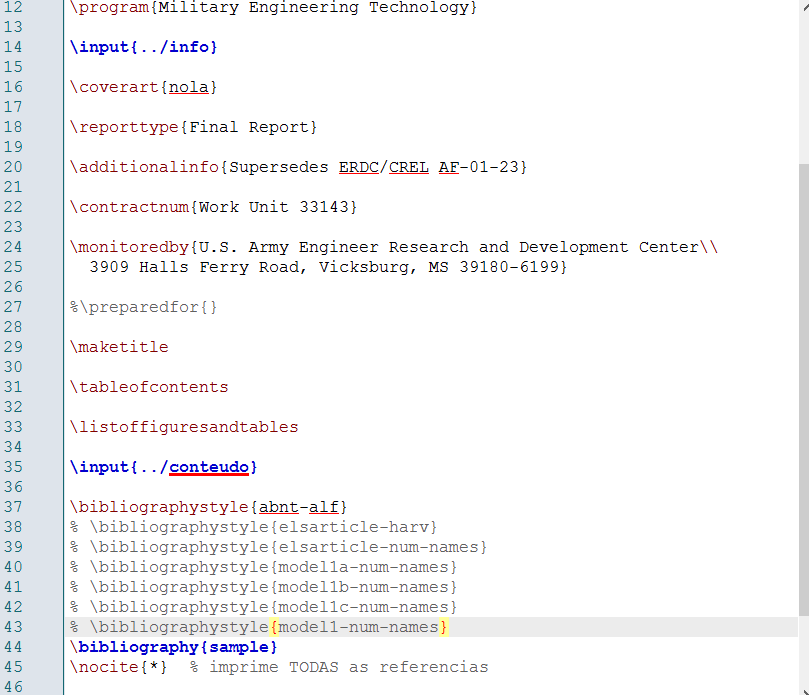
\includegraphics[scale=0.4]{figuras/armyInputs.png}
\caption{Inputs para uso genério de templates (Army Eng)}
\end{center}
\end{figure}
\end{frame}

\begin{frame}
\begin{figure}
Observe os comandos de \textbackslash input e \textbackslash bibliography nos arquivos tex internos de cada template:
\begin{center}
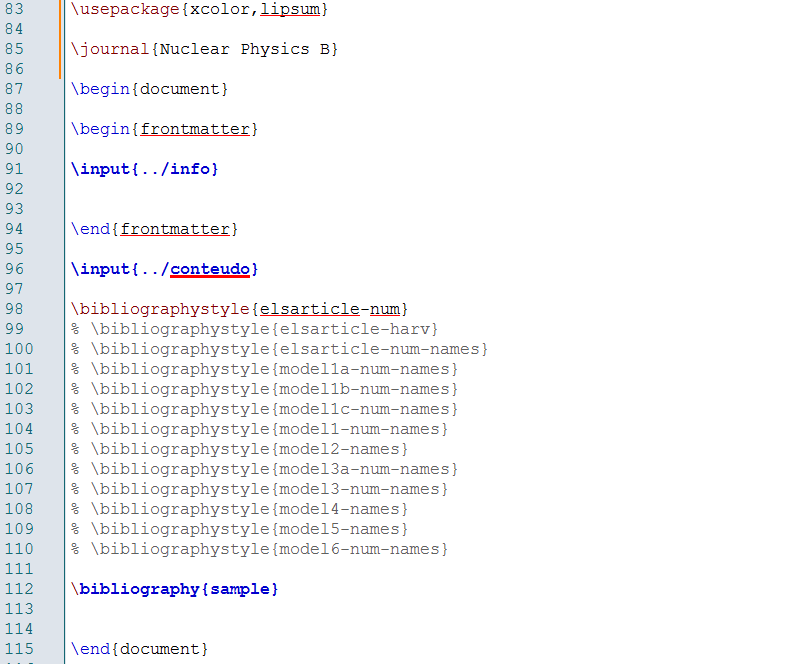
\includegraphics[scale=0.4]{figuras/cicInputs.png}
\caption{Inputs para uso genério de templates (Procedia)}
\end{center}
\end{figure}
\end{frame}


\begin{frame}[fragile]
Compilar \textit{F6}, gerar referencia bibliográfica \textit{F11},  Compilar \textit{F6} e visualizar o resultado \textit{F7}.
\end{frame}





